
\section{Support Vector Machines}

\textit{Support Vector Machines} (SVM), are one of the most popular models in Machine Learning. SVMs are capable of 
performing linear or nonlinear classification, regression and outlier detection. In general, SVMs are particularly 
strong suited in classification tasks that include complex datasets that are small or medium sized, as they do 
not scale well into larger datasets.

\subsection{How SVMs Work}

In this section we will be covering the mechanics behind how SVMs make predictions and how their training algorithms
work. A few words on notations, the bias terms will be called \textit{b}, and the feature weights vector will be 
called $\vec{w}$. Additionally, no bias feature will be added to the input feature vectors.

\subsubsection*{Decision Function and Predictions}

A linear SVM classifier model predicts the class of a new instance $\vec{x}$ by simply computing the
decision function: $\vec{w}^{\intercal}\vec{x} + b = w_{1}x_{1} + \cdots + w_{n}x_{n} + b$. If the result is 
positive, the predicted class $\hat{y}$ is the positive class (1), and otherwisw it is the negative class (0).
Below will be the function for a Linear SVM classifer's predictions:

\[ \hat{y} = 
\begin{cases} 
    0 & \text{if } \vec{w}^{\intercal}\vec{x} + b < 0 \\
    1 & \text{if } \vec{w}^{\intercal}\vec{x} + b \geq 0
\end{cases}
\] \\

\noindent
The figure below will show the plot of the decision function. It is a 2D plane because the dataset we are 
training the model on has only 2 features: petal width and petal length (Iris Datset). The decision boundary
is the set of points where the decision function is equal to 0: it is the intersection of 2 planes, which 
is a straight line (represented by the thick solid line).

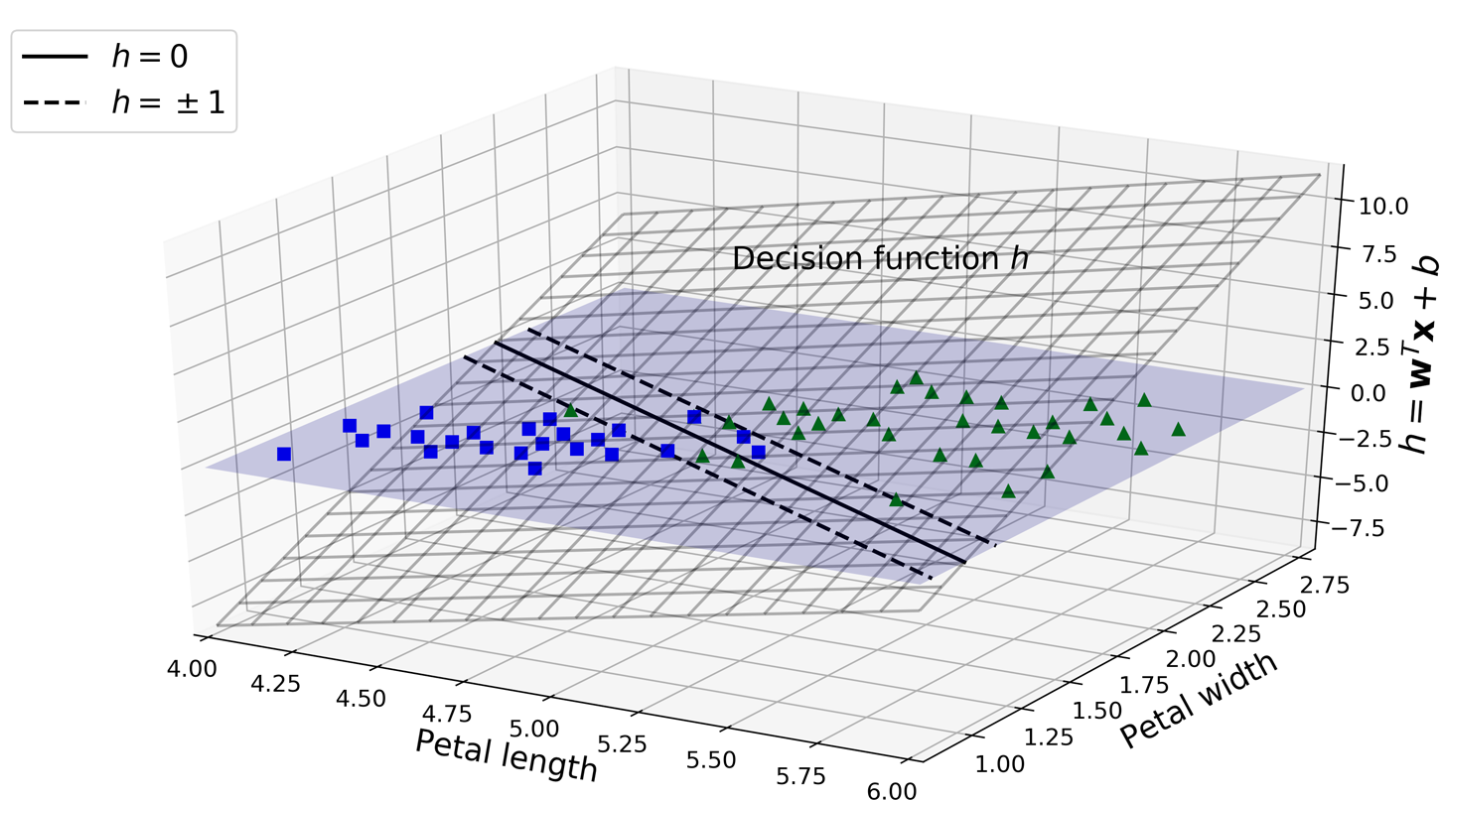
\includegraphics[scale=0.65]{Images/svm_DecisionFunc.PNG}

\noindent
The dashed lines represent the points where the decision function is equal to 1 or -1. \textbf{Note:}
they are parallel and at equal distance to the decision boundary, and they form a margin around
it. When we train a linear SVM classifier, we are finding the values of $\vec{w}$ and $b$ that 
make this margin as wide as possible while avoiding margin violations (\textit{hard margin}) 
or limiting them (\textit{soft margin}). 

\subsubsection*{Training Objective}

Consider the norm of the weight vector, $\norm{\vec{w}}$, we find that it is equivalent to the slope of the
decision function. If we were to divide this slope by 2, we will also find that the points where the decision
function is equal to $\pm 1$ are going to twice as far away from the decision boundary. This can be seen in the 
figure below:

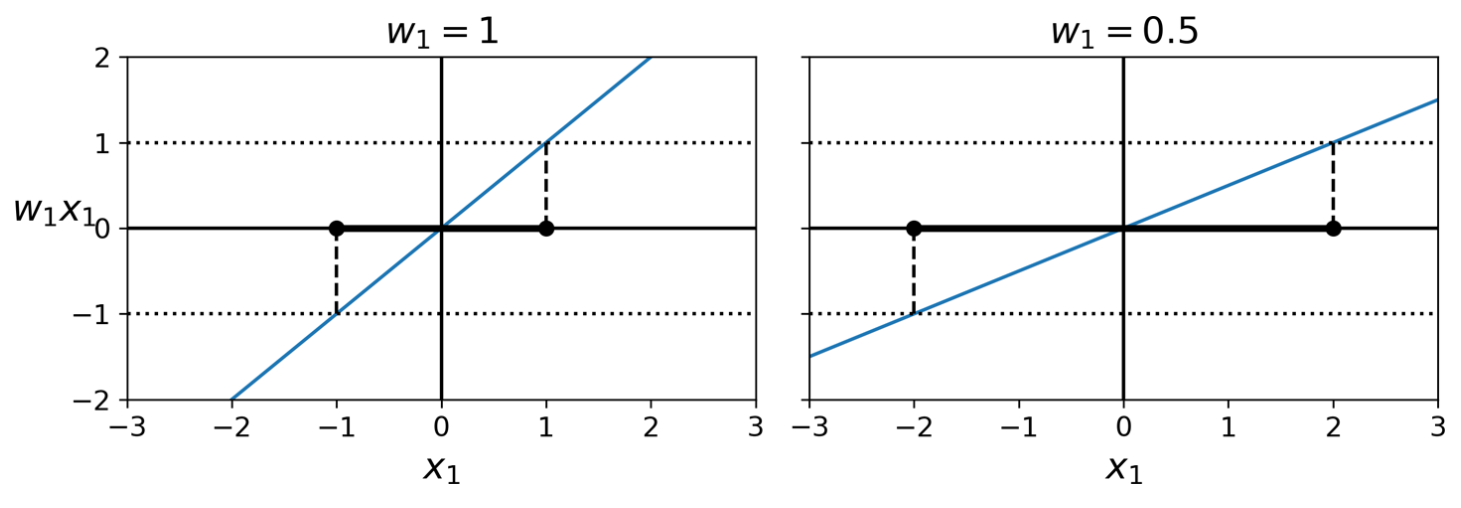
\includegraphics[scale=0.65]{Images/weightVec.PNG}

\noindent
Therefore, we want to minimize $\norm{\vec{w}}$ to get the largest possible margin. Additionally, if we want to
avoid any margin violations (hard margin), then we need the decision function to be greater than 1 for all 
positive training instances and lower than -1 for negative training instances. \\

\noindent
Further, if we define $t^{(i)} = -1$ for negative instance (if $y^{(i)} = 0$) and $t^{(i)} = 1$ for positive
instances (if $y^{(i)} = 1$), then we can express the constraint as $t^{(i)}(\vec{w}^{\intercal}\vec{x}^{(i)}+b) \geq 1$
for all instances.\\

\noindent
Finally, we can express the \textbf{hard margin} linear SVM classifier objective as the constrained optimization 
problem below:

\[
\begin{aligned}
\min_{\vec{w},b} \quad & \frac{1}{2}\vec{w}^{\intercal}\vec{w}\\
\textrm{subject to:} \quad & t^{(i)}(\vec{w}^{\intercal}\vec{x}^{(i)}+b) \geq 1 & \textrm{for } i = 1, 2, \cdots, m
\end{aligned}
\] \\

\noindent
\textbf{Note:} We are minimizing $\frac{1}{2} \vec{w}^{\intercal}\vec{w}$, which is just equal to 
$\frac{1}{2} \norm{\vec{w}}^{2}$, rather than minimizing $\norm{\vec{w}}$. This is because $\frac{1}{2} \norm{\vec{w}}^{2}$
has a nice derivative, which is just $\vec{w}$, whereas $\norm{\vec{w}}$ is not differentiable at $\vec{w} = 0$. 
In general optimization algorithms work much better on differentiable functions.\\

\noindent
For the \textbf{soft margin} objective, we need to a \textit{slack variable} $\zeta^{(i)} \geq 0$ for each 
instance. $\zeta^{(i)}$ can be described as how much the $i^{th}$ instace is allowed to violate the margin
(decision boundary). However, now we have two conflicting objectives:

\begin{itemize}
    \item First, is to minimize the slack variables as much as possible to reduce the margin violations
    \item Second, make $\frac{1}{2} \vec{w}^{\intercal}\vec{w}$ as small as possible to increase the margin
\end{itemize}

\noindent
Finally, this is where the \mintinline{python}{C} hyperparameter comes in. This hyperparameter allows us to 
define the tradeoff between these two objectives, thus, giving us the constrained optimization problem for 
the \textbf{soft margin} linear SVM classifier:

\[
\begin{aligned}
\min_{\vec{w},b, \zeta} \quad & \frac{1}{2}\vec{w}^{\intercal}\vec{w} + C\sum^{m}_{i=1} \zeta^{(i)}\\
\textrm{subject to:} \quad & t^{(i)}(\vec{w}^{\intercal}\vec{x}^{(i)}+b) \geq 1 - \zeta^{(i)} & \textrm{ for } i = 1, 2, \cdots, m\\
                           & \zeta^{(i)} \geq 0
\end{aligned}
\]

\subsubsection*{Quadratic Programming}

Hard and Soft Margin problems are both convex quadratic optimization problems with linear constraints. This is 
commonly known as \textit{Quadratic Programming} (QP) problems. There are many algorithms that can be used
for this task. Take a look at this \changeurlcolor{blue}\href{https://web.stanford.edu/~boyd/cvxbook/bv_cvxbook.pdf}{book} for more 
detailed explanations of these algorithms. \\

\noindent
The general Quadratic Programming problem to solve is given by:

\[
\begin{aligned}
\min_{\vec{p}} \quad & \frac{1}{2}\vec{p}^{\intercal}\vec{H}\vec{p} + \vec{f}^{\intercal}\vec{p}\\
\textrm{subject to:} \quad & \vec{A}\vec{p} \leq \vec{b} \\
\textrm{where} \quad & 
\begin{cases} 
    \vec{p} & \textrm{ is an } n_{p}-\textrm{dimensional vector } (n_{p} = \textrm{ number of parameters}) \\
    \vec{H} & \textrm{ is an } n_{p} \times n_{p} \textrm{ matrix} \\
    \vec{f} & \textrm{ is an } n_{p}-\textrm{dimensional vector} \\
    \vec{A} & \textrm{ is an } n_{c} \times n_{p} \textrm{ matrix } (n_{c} = \textrm{ number of constraints})\\
    \vec{b} & \textrm{ is an } n_{c}-\textrm{dimensional vector}
\end{cases}
\end{aligned}
\] \\

\noindent 
Note that the expression $\vec{A}\vec{p} \leq \vec{b}$ defines a $n_{c}$ constraints: $\vec{p}^{\intercal}\vec{a}^{(i)} \leq b^{(i)}$
for $i = 1, 2, \cdots, n_{c}$, where $\vec{a}^{(i)}$ is the vector containing the elements of the $i^{th}$ row
of $\vec{A}$ and $b^{(i)}$ is the $i^{th}$ element of $\vec{b}$.\\

\noindent 
As an example, we can verify the QP parameters for a hard margin linear SVM classifier below:

\begin{itemize}
    \item $n_{p} = n + 1$, where $n$ is the number of features (+1 is for the bias term)
    \item $n_{c} = m$, where $m$ is the number of training instances
    \item $\vec{H}$ is the $n_{p} \times n_{p}$ identity matrix, except with a zero in the top-left cell (to ignore the bias term)
    \item $\vec{f} = 0$, an $n_{p}-$dimensional vector full of 0s
    \item $\vec{b} = -1$, an $n_{c}-$dimensional vector full of -1s
    \item $\vec{a}^{(i)} = -t^{(i)}\dot{\vec{x}}^{(i)}$, where $\dot{\vec{x}}^{(i)}$ is equal to $\vec{x}^{(i)}$ with an extra bias feature $\dot{\vec{x}}_{0} = 1$
\end{itemize}

\noindent
Thus, one way to train a hard margin linear SVM classifier is to use an off-the-shelf QP solver and pass it the 
preceding parameters. The resulting vector $\vec{p}$ will contain the bias term $b = p_{0}$ and the feature 
weights $w_{i} = p_{i}$ for $i = 1, 2, \cdots, n$. Similarily, we can solve the soft margin problem using 
a QP solver as well. 

\subsubsection*{The Dual Problem}

For more indepth explanation of this problem reference \changeurlcolor{blue}\href{https://en.wikipedia.org/wiki/Duality_(optimization)}{this site}.\\

\noindent
In its most basic form the \textit{Dual Problem (Duality)} is when we have a given constrained optimization
problem, known as the \textit{primal problem}, and it is possible to express a different but closely related 
problem, called the \textit{dual problem}. Typically, the dual problem gives a lower bound to the solution of the 
primal problem. \\

\noindent
Fortunately, the SVM constrained optimization problem meets these conditions, so we have the choice to solve the 
primal or dual problem. The optimal solutions for both will be the same. To derive the unconstrained optimization
problem for the hard margin SVM, we need to use \textit{Lagrange Multipliers}. \\

\noindent
Given the constraints we shown earlier, we can write down the \textit{Generalized Lagrangian} for the hard margin
problem for linear SVMs. $\alpha^{(i)}$, is the variable that is called the \textit{Karush-Kuhn-Tucker} (KKT)
multipliers. Below will be the Lagrangian:

\[
\begin{aligned}
\mathcal{L}(\vec{w}, b, \alpha) = \frac{1}{2}\vec{w}^{\intercal}\vec{w} - \sum_{i=1}^{m} \alpha^{(i)}(t^{(i)}(\vec{w}^{\intercal}\vec{x}^{(i)} + b) - 1)\\
\textrm{with } \alpha^{(i)} \geq 0 \textrm{ for } i = 1, 2, \cdots, m
\end{aligned}
\]\\

\noindent
As follows with Lagrange multipliers, we can compute the partial derivatives and locate the optimal points. If
there is a solution, it will be among the stationary points $(\hat{\vec{w}}^{\intercal}, \hat{b}, \hat{\alpha})$ 
that respect the KKT Conditions:

\begin{itemize}
    \item Respect the problems constraints: $t^{(i)}(\vec{w}^{\intercal}\vec{x}^{(i)}+b) \geq 1 \textrm{ for } i = 1, 2, \cdots, m$
    \item Verify $\hat{\alpha}^{(i)} \geq 0 \textrm{ for } t = 1,2, \cdots, m$
    \item Either $\hat{\alpha}^{(i)} = 0$ or the $i^{th}$ constraint must be an \textit{active constraint}, meaning it
    must hold by equality: $t^{(i)}(\vec{w}^{\intercal}\vec{x}^{(i)}+b) = 1$. This condition is called the 
    \textit{complementrary slackness} condition. It implied that either $\hat{\alpha}^{(i)} = 0$ or the 
    $i^{th}$ instance lies on the boundary (it is a support vector).
\end{itemize}

\noindent 
\textbf{Note} that the KKT conditions are necessary conditions for a stationary point to be a solution of the 
constrained optimization problem. Fortunately, the SVM optimization problem meets all these conditions, so any
stationary point that meets the KKT conditions is guaranteed to be a solution to the constrained optimization 
problem.\\

\noindent
We can compute the partial derivatives of the generalized Lagrangian with regard to $\vec{w}$ and $b$:

$$\nabla_{\vec{w}} \mathcal{L}(\vec{w}, b, \alpha) = \vec{w} - \sum_{i=1}^{m} \alpha^{(i)}t^{(i)}\vec{x}^{(i)}$$

$$\frac{\partial}{\partial b}\mathcal{L}(\vec{w}, b, \alpha) = -\sum_{i=1}^{m} \alpha^{(i)}t^{(i)}$$

\noindent
We then set these partial derivatives equal to zero, and we can get the following:

$$\hat{\vec{w}} = \sum_{i=1}^{m} \hat{\alpha}^{(i)} t^{(i)} \vec{x}^{(i)}$$

$$\sum_{i=1}^{m} \hat{\alpha}^{(i)} t^{(i)} = 0$$

\noindent
Now we can plug these results into the definition of the generalized Lagrangian and we get the following dual 
problem form for the SVM problem:

\[
\begin{aligned}
\mathcal{L}(\hat{\vec{w}}, \hat{b}, \alpha) = \frac{1}{2} \sum_{i=1}^{m} \sum_{j=1}^{m} \alpha^{(i)} \alpha^{(j)} t^{(i)} t^{(j)} \vec{x}^{(i)\intercal} \vec{x}^{(j)} - \sum_{i=1}^{m} \alpha^{(i)} \\
\textrm{with } \alpha^{(i)} \geq 0 \textrm{ for } i = 1, 2, \cdots, m
\end{aligned}
\] \\

\noindent
We now want to find the vector $\hat{\vec{\alpha}}$, that minimizes this function, while $\hat{\alpha}^{(i)} \geq 0$
for all instances. \\

\noindent
Once we find the optimal $\hat{\vec{\alpha}}$, we can compute $\hat{\vec{w}}$ using the partial derivative w.r.t. 
$\vec{w}$ of the Lagrangian. To compute $\hat{b}$, we can use the fact that a support vector must satisfy 
$t^{(i)}(\hat{\vec{w}}^{\intercal}\vec{x}^{(i)}+\hat{b}) = 1$, so if the $k^{th}$ instance is a support vector
(i.e., $\hat{\alpha}^{(k)} > 0$), we can use it to compute $\hat{b} = t^{(k)} - \hat{\vec{w}}^{\intercal}\vec{x}^{(k)}$.
However, it is often preferred to compute the average over all support vectors to get a more stable and 
precise value as show below: (Bias term estimation using the dual form)

$$\hat{b} = \frac{1}{n_{s}} \sum_{\substack{i = 1 \\ \hat{\alpha}^{(i)}>0}}^{m} [t^{(i)} - \hat{\vec{w}}^{\intercal}\vec{x}^{(i)}]$$

\noindent
Altogether it is found that the dual problem is faster to solve than the primal one when the number of training
instances is smaller than the number of features. However, more importantly the dual problem allows us to use 
something called the \textit{kernel trick} prossible, while the primal does not (More explained in next section).

\subsubsection*{Kernelized SVMs}

Suppose we want to apply a second-degree polynomial transformation to a two-dimensional training set, then train a 
linear SVM classifier on the transformed training set. Below we can see the second-degree polynomial mapping 
function $\boldsymbol{\phi}$ we want to apply:

$$\boldsymbol{\phi}(\vec{x}) = 
\boldsymbol{\phi}
\begin{pmatrix}
    \begin{pmatrix}
        x_{1} \\
        x_{2}
    \end{pmatrix}
\end{pmatrix}
= 
\begin{pmatrix}
    x_{1}^{2} \\
    \sqrt{2}x_{1}x_{2} \\
    x_{2}^{2}
\end{pmatrix}
$$ \\

\noindent
\textbf{Notice:} that the transformed vector is 3D instead of 2D. Now we take a look at how 2D vectors, $\vec{a}$ and 
$\vec{b}$, if we apply this second-degree polynomial mapping and then compute the dot product of the transformed 
vectors we get the following:

\[
\begin{aligned}
\boldsymbol{\phi}(\vec{a})^{\intercal}\boldsymbol{\phi}(\vec{b}) = 
\begin{pmatrix}
    a_{1}^{2} \\
    \sqrt{2}a_{1}a_{2} \\
    a_{2}^{2}
\end{pmatrix}
^{\intercal}
\begin{pmatrix}
    b_{1}^{2} \\
    \sqrt{2}b_{1}b_{2} \\
    b_{2}^{2}
\end{pmatrix}
=
a_{1}^{2}b_{1}^{2} + 2a_{1}b_{1}a_{2}b_{2} + a_{2}^{2} b_{2}^{2}\\
= (a_{1}b_{1} + a_{2}b_{2})^{2} = 
\begin{pmatrix}
    \begin{pmatrix}
        a_{1}\\
        a_{2}
    \end{pmatrix}
    ^{\intercal}
    \begin{pmatrix}
        b_{1} \\
        b_{2}
    \end{pmatrix}
\end{pmatrix}
^{2} = 
(\vec{a}^{\intercal}\vec{b})^{2}
\end{aligned}
\]

\noindent
From the above, we can see that the dot product of the transformed vectors is equal to the sum of the square of the 
dot product of the original vectors 
$\boldsymbol{\phi}(\vec{a})^{\intercal}\boldsymbol{\phi}(\vec{b}) = (\vec{a}^{\intercal}\vec{b})^{2}$.\\

\noindent
\textbf{Key Insight:} if we want to apply the transformation $\boldsymbol{\phi}$ to all training instances, then
the dual problem (mentioned earlier), will be the dot product 
$\boldsymbol{\phi}(\vec{x}^{(i)})^{\intercal}\boldsymbol{\phi}(\vec{x}^{(j)})$. But if $\boldsymbol{\phi}$ is 
the second-degree polynomial transformation defined earlier, then we can replace this dot product of the 
transformed vectors simply by $(\vec{x}^{(i)\intercal}\vec{x}^{(j)})^{2}$. Therefore, we do not need to transform
the training instances at all; just replace the dot product by its square in the dual problem for SVM defined 
earlier. The following result will be the same as if we went through the trouble of transforming the training 
set then fitting a linear SVM algorithm, however, this "trick" makes the process much more computationally
efficient. \\

\noindent
In Machine Learning, a \textit{kernel} is a function capable of computing the dot product 
$\boldsymbol{\phi}(\vec{a}^{\intercal})\boldsymbol{\phi}\vec{b}$, based only on the original vectors $\vec{a}$ 
and $\vec{b}$, without having to compute (or even know) the transformation $\boldsymbol{\phi}$. Below will be a 
list of some of the most commonly used kernels:

\[
\begin{aligned}
\textrm{Linear:} \quad & K(\vec{a}, \vec{b}) = \vec{a}^{\intercal}\vec{b} \\
\textrm{Polynomial:} \quad & K(\vec{a}, \vec{b}) = (\gamma\vec{a}^{\intercal}\vec{b} + r)^{d} \\
\textrm{Gaussian RBF:} \quad & K(\vec{a}, \vec{b}) = \textrm{exp}(-\gamma \norm{\vec{a} - \vec{b}}^{2}) \\
\textrm{Sigmoid:} \quad & K(\vec{a}, \vec{b}) = \textrm{tanh}(\gamma\vec{a}^{\intercal}\vec{b} + r)
\end{aligned}
\] \\

\noindent
\textbf{Mercer's Theorem:} According to this theorem if a function $K(\vec{a}, \vec{b})$ respects a few 
mathematical conditions called \textit{Mercer's Conditions} (e.g., K must be continous and symmertric in its 
arguements so that $K(\vec{a}, \vec{b}) = K(\vec{b}, \vec{a})$, etc.), then there exists a function 
$\boldsymbol{\phi}$ that maps $\vec{a}$ and $\vec{b}$ into another space (possible with much higher dimensions) 
such that $K(\vec{a}, \vec{b}) = \boldsymbol{\phi}(\vec{a})^{\intercal} \boldsymbol{\phi}(\vec{b})$. We can use 
K as a kernel because we know that $\boldsymbol{\phi}$ exists, even if we dont know exactly what 
$\boldsymbol{\phi}$ is. For example int he case of the Gaussian RBF kernel, it can be shown that 
$\boldsymbol{\phi}$ maps each training instance to an infinite-dimensional space.\\

\noindent
Note, that some frequently used kernels (such as the sigmoid kernel) do not respect all of the Mercer's conditions,
yet they generally work well in practice. \\

\noindent
Earlier in this section we covered how to get to the dual solution to the primal solution in the case of the 
linear SVM classifier. But if we were to apply the kernel trick, we will end up with equations that include
$\boldsymbol{\phi}(x^{(i)})$, which may be large or even infinite, so we are not able to compute it. Then we 
ask the question how can we make predictions without knowing $\vec{\hat{w}}$? Well we can plug in $\vec{\hat{w}}$
from the partial derivatives we took earlier, into the decision function for a new instance $\vec{x}^{(n)}$, and
we get an equation with only dot products between input vectors. This is what makes it possible to use the kernel
trick. Below will be how we make predictions with a kernelized SVM:

\begin{eqnarray}
h_{\vec{\hat{w}}, \vec{\hat{b}}}\left(\boldsymbol{\phi}(\vec{x}^{n})\right) &=& \vec{\hat{w}}^{\intercal}\boldsymbol{\phi}\left(\vec{x}^{(n)}\right) + \hat{b} =\left(\sum_{i=1}^{m} \hat{\alpha}^{(i)}t^{(i)}\boldsymbol{\phi}\left(\vec{x}^{(i)}\right)\right)^{\intercal}\boldsymbol{\phi}\left(\vec{x}^{(n)}\right) + \hat{b} \nonumber \\
                                                                 &=& \sum_{i=1}^{m} \hat{\alpha}^{(i)}t^{(i)} \left(\boldsymbol{\phi}\left(\vec{x}^{(i)}\right)^{\intercal}\boldsymbol{\phi}\left(\vec{x}^{(n)}\right)\right) + \hat{b} \nonumber \\
                                                                 &=& \sum_{\substack{i=1 \\ \hat{\alpha}^{(i)} > 0}}^{m} \hat{\alpha}^{(i)} t^{(i)} K\left(\vec{x}^{(i)}, \vec{x}^{(n)}\right) + \hat{b} \nonumber
\end{eqnarray}

\noindent
Note that since $\alpha^{(i)} \neq 0$ only for support vectors, making predictions involves computing the dot
product of the new input vector $\vec{x}^{(n)}$ with only the support vectors, not all the training instances.
Additionally, we will use the same trick to compute the bias term $\hat{b}$:

\begin{eqnarray}
\hat{b} &=& \frac{1}{n_{s}} \sum_{\substack{i=1 \\ \hat{\alpha}^{(i)} > 0}}^{m} \left(t^{(i)} - \vec{\hat{w}}^{\intercal}\boldsymbol{\phi}\left(\vec{x}^{(i)}\right)\right) \nonumber \\
        &=& \frac{1}{n_{s}} \sum_{\substack{i=1 \\ \hat{\alpha}^{(i)} > 0}}^{m} \left(t^{(i)} - \left(\sum_{j=1}^{m} \hat{\alpha}^{(j)}t^{(j)}\boldsymbol{\phi}\left(\vec{x}^{(j)}\right)\right)^{\intercal} \boldsymbol{\phi}\left(\vec{x}^{(i)}\right)\right) \nonumber \\
        &=& \frac{1}{n_{s}} \sum_{\substack{i=1 \\ \hat{\alpha}^{(i)} > 0}}^{m} \left(t^{(i)} - \sum_{\substack{j=1 \\ \hat{\alpha}^{(j)}}}^{m} \hat{\alpha}^{(j)}t^{(j)} K\left(\vec{x}^{(i)}, \vec{x}^{(j)}\right)\right) \nonumber
\end{eqnarray}

\noindent
Finally, we have finished understanding the inner workings of the kernelized SVM. 

\subsection{Linear SVM Classification}
The fundamental idea behind \textit{Support Vector Machines} is to find a line that can separate two separate 
classes (Data would be known as \textit{linearly separable}). The goal of a SVM classifier is to find a way to 
separate the two classes, but to simultaneously also fit the widest possible street for separating the two 
classes. This is called \textit{Large Margin Classification}.\\

\noindent
\textbf{Note:} adding more training instaces that are "off the street" will not affect the decision boundary at
all. The decision boundary is determined (or "supported) by the instances located on the edge of the street only. 
These instances are called the \textit{support vectors}. \\ 

\noindent
\textbf{Important}, SVMs are sensitive to feature scaling, so we must be wary when we are training models on 
unscaled data or when we are doing any feature engineering.

\subsubsection{Hard Margin Classification}

\textit{Hard Margin Classification} is when we are looking to very strict with the classification of our instances.
We can impose a rule there all instances must be off the decision boundary and on the right side. This is the 
basic rule of hard margin classification. \\

\noindent
However there are two main issues that are associated with this type of classification:

\begin{itemize}
    \item This type of classification \textbf{only} works if the data is linearly separable.
    \item Training a model like this is also very sensitive to outliers. For example, with just one outlier 
    on the wrong side of the class will make it impossible for there to be a hard margin. This will also likely
    lead to having the model generalize very poorly.     
\end{itemize}

\noindent
Therefore, in most cases it is not preferred to use hard margin classification when training a SVM as it is not
able to handle many real world datasets.

\subsubsection{Soft Margin Classification}

On the other hand, \textit{Soft Margin Classification} is a much more flexible classification system. Here the 
objective is to find the right balance between keeping the decision boundary as large as possible and limiting the 
\textit{margin violations} (i.e., instances that end up in the middle of the boundary or on the wrong side). \\

\noindent
When creating a SVM model using Scikit-Learn, there is a hyperparameter \mintinline{python}{C} that allows us to 
regularize the model. If we set a low value for \mintinline{python}{C}, then we end up with a more flexible model,
whereas, if we set a high \mintinline{python}{C}, then we get a model that much more similar to 
\textit{hard margin classification}.

\subsubsection*{Example of SVM in Python}

The following code will be using Scikit-Learn to train a linear SVM model on the iris dataset. The code will scale 
the features and then train the model. The objective of this model it to detect \textit{Iris Virginica} flowers in
the iris dataset. 

\begin{minted}{python}
import numpy as np
from sklearn import datasets
from sklearn.pipeline import Pipeline
from sklearn.preprocessing import StandardScaler
from sklearn.svm import Linear SVC

iris = datasets.load_iris() # Iris Dataset
X = iris["data"][:, (2, 3)] # Petal Length, Petal Width
y = (iris["target"] == 2).astype(np.float64) # Iris Virginica

svm_clf = Pipeline([
            ("Scaler", StandardScaler()),
            ("linear_svc", LinearSVC(C=1, loss="hinge")),
    ])

svm_clf.fit(X, y)

svm_clf.predict([[5.5, 1.7]])
# Output: array([1.])
\end{minted}

\noindent
Additionally, instead of using the \mintinline{python}{LinearSVC} class, we can also use the \mintinline{python}{SVC}
class with a linear kernel. When creating the SVC model, we will just need to specify \mintinline{python}{SVC(kernel="linear", C=1)}.

\subsection{Non-Linear SVM Classification}

There are many times when datasets are not anywhere close to being linearly separable. In this section we will be covering different
ways to go about creating nonlinear SVM classifiers. The first approach is to add more features, such as polynomial features, which
in some cases may lead to the dataset being linearly separable. As an example below we have 2 graphs, on the left there is just one 
variable, $x_{1}$, and we can clearly see that the data is not linearly separable. Now on the right graph, we add a second feature
$x_{2} = (x_{1})^{2}$, resulting in a 2D dataset that is perfectly linearly separable. \\

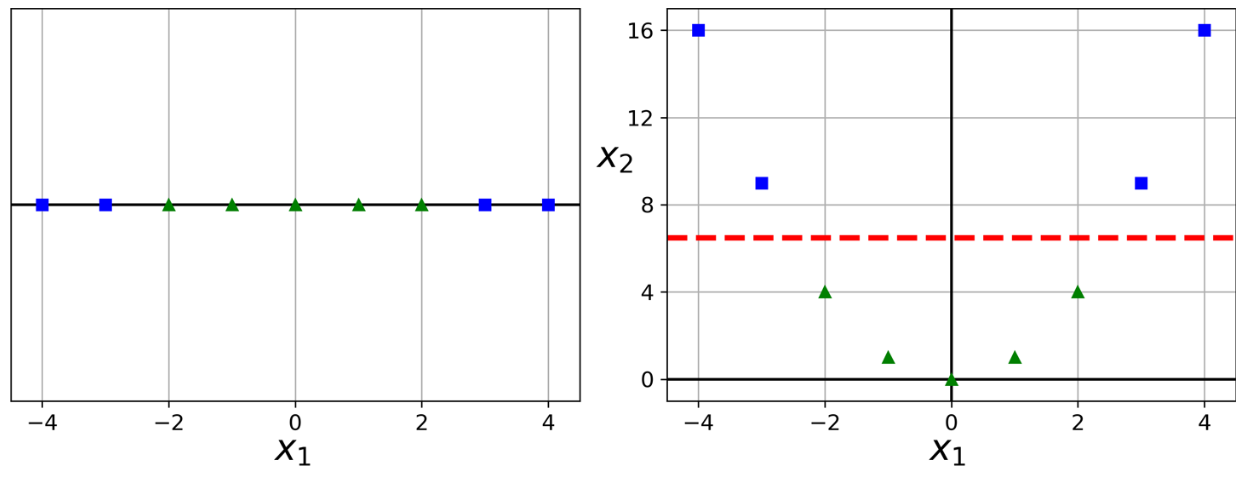
\includegraphics[scale=0.45]{Images/linearSeparable.PNG}

\noindent
To implement this using Scikit-Learn, we can create a \mintinline{python}{Pipeline} containing \mintinline{python}{PolynomialFeatures}
transformer, followed by a \mintinline{python}{StandardScaler} and a \mintinline{python}{LinearSVC}. The example below will be used 
on the moons dataset: this is a toy dataset for binary classification in which the data points are shaped as two interleaving 
half circles. Below will be the code:

\begin{minted}{python}
from skelarn.datasets import make_moons
from sklearn.pipeline import Pipeline
from sklearn.preprocessing import PolynomialFeatures, StandardScaler

X, y = make_moons(n_samples=100, noise=0.15)
polynomial_svm_clf = Pipeline([
        ("poly_features", PolynomialFeatures(degree=3)),
        ("scaler", StandardSCaler()),
        ("svm_clf", LinearSVC(C=10, loss="hinge"))
    ])

polynomial_svm_clf.fit(X, y)
\end{minted}

\noindent
Additionally, below we can see what the decision boundary of the polynomial SVM classifier looks like on the moons dataset.\\

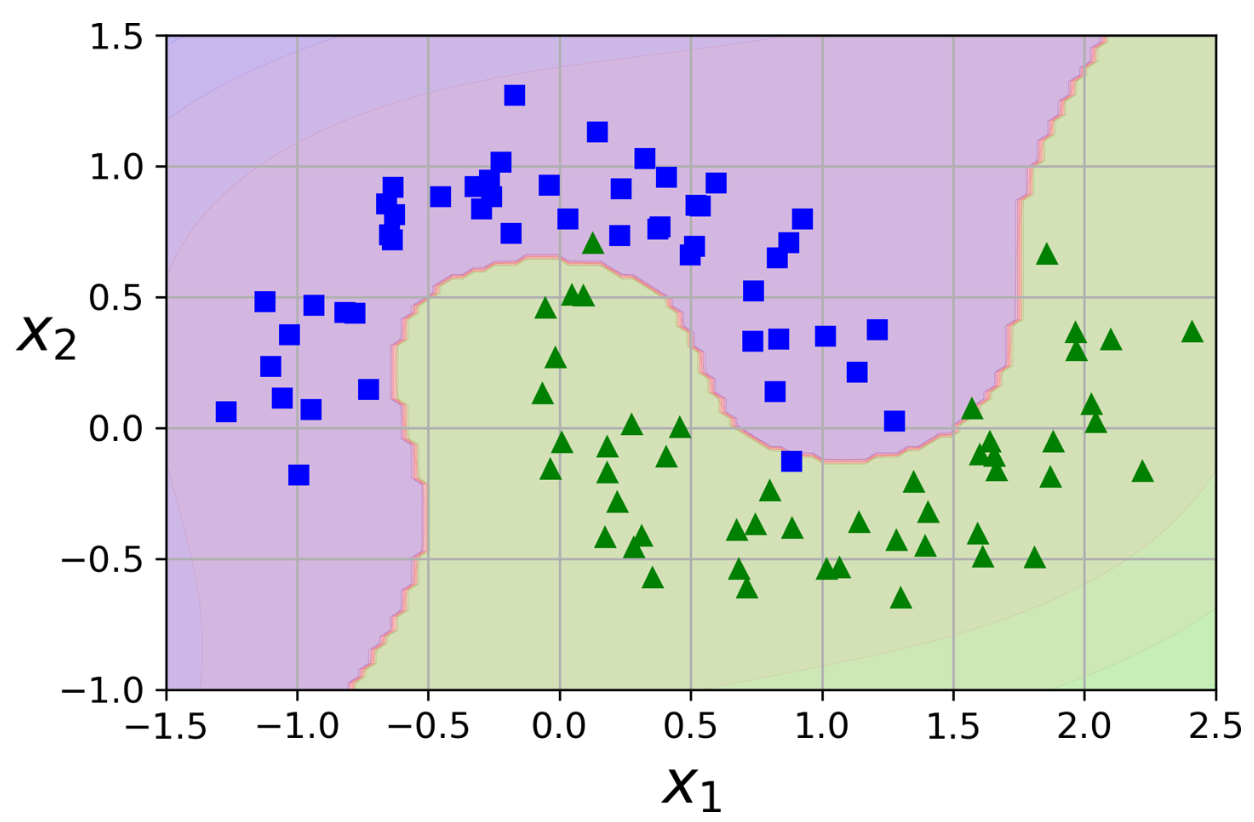
\includegraphics[scale=0.4]{Images/nonlinearSVM.PNG}

\subsubsection{Polynomial Kernel}

As seen above adding polynomial features is simple and quite easy to implement. However, at a low polynomial degree, this method does
not have the ability to deal with very complex datasets, and with high degree polynomials it creates a huge number of features 
making model training too slow. \\

\noindent
Fortunately, for SVMs, we can use the \textit{kernel trick}. As explained earlier, this trick makes it possible to get the same result
as if we had added many polynomial features, without having to actually add them into the model. This trick is already built into the 
\mintinline{python}{SVC} class. Below will be testing it on the moons dataset:

\begin{minted}{python}
from sklearn.svm import SVC
poly_kernel_svm_clf = Pipeline([
        ("scaler", StandardScaler()),
        ("svm_clf", SVC(kernel="poly", degree=3, coef0=1, C=5))
    ])

poly_kernel_svm_clf.fit(X, y)
\end{minted}

\noindent
In the code above, we are training a polynomial SVM using the kernel trick. Specifically in this case, we are training a 3-degree 
polynomial SVM classifier.\\

\noindent
In the graphic below, we can see the 3-degree polynomial
model on the left and on the right there is another 10-degree polynomial kernel. The hyperparameter \mintinline{python}{coef0} controls
how much the model is influenced by high-degree polynomials versus low-degree polynomials.\\

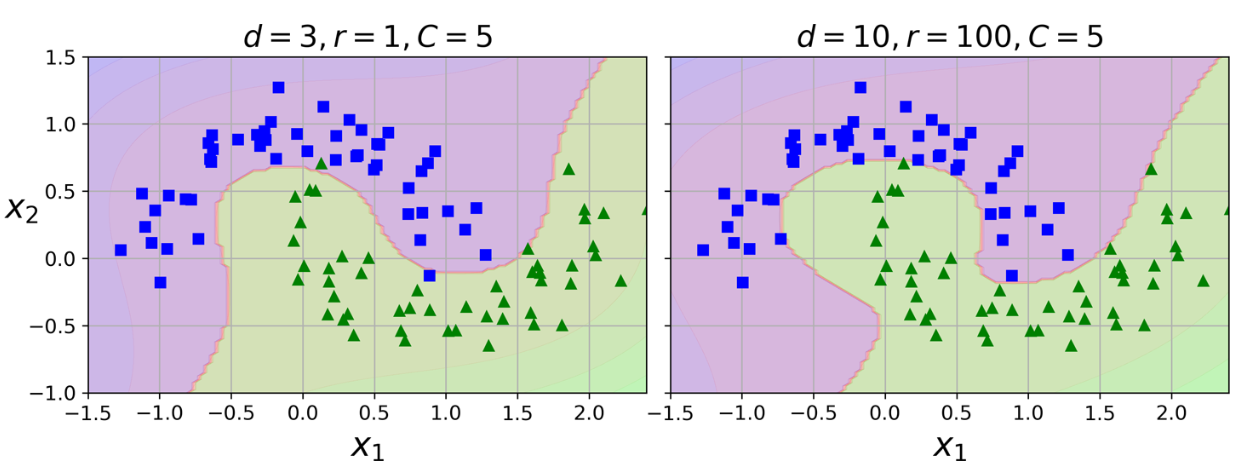
\includegraphics[scale=0.45]{Images/polyKernel.PNG}

\noindent
\textbf{Note:}, generally it is common practice to use grid search when trying to find the right hyperparameter values. It is fastest to 
first do a very coarse grid search, and then a finer grid search around the best values found. 

\subsubsection{Gaussian RBF Kernel}

Once again we can use the \textit{kernel trick} to reduce the computational expensiveness to compute all the additional features if we 
were to add all the similarity features manually. Below will be the implementation of \mintinline{python}{SVC} class with the 
Gaussian RBF Kernel:

\begin{minted}{python}
rbf_kernel_svm_clf = Pipeline([
        ("scaler", StandardScaler()),
        ("svm_clf", SVC(kernel="rbf", gamma=5, C=0.001))
    ])

rbf_kernel_svm_clf.fit(X, y)
\end{minted}

\noindent
Below will be a graphic showing different decision boundaries of the Gaussian RBF Kernel for varying values of \mintinline{python}{gamma}
($\gamma$) and \mintinline{python}{C}. Increasing \mintinline{python}{gamma} makes the bell-shaped curve narrower. As a result, each
instance's range of influence is smaller, in other words, the decision boundary ends up being more irregular, wiggling around individual
instances. Conversely, a small \mintinline{python}{gamma} value makes the bell-shaped curve wider, therefore, instances have a larger
range of influence, and the decision boundary ends up smoother. So $\gamma$ acts like a regularization hyperparameter: if we have a model
that is overfitting, we should reduce $\gamma$ and if it is underfitting, we should increase $\gamma$. \\

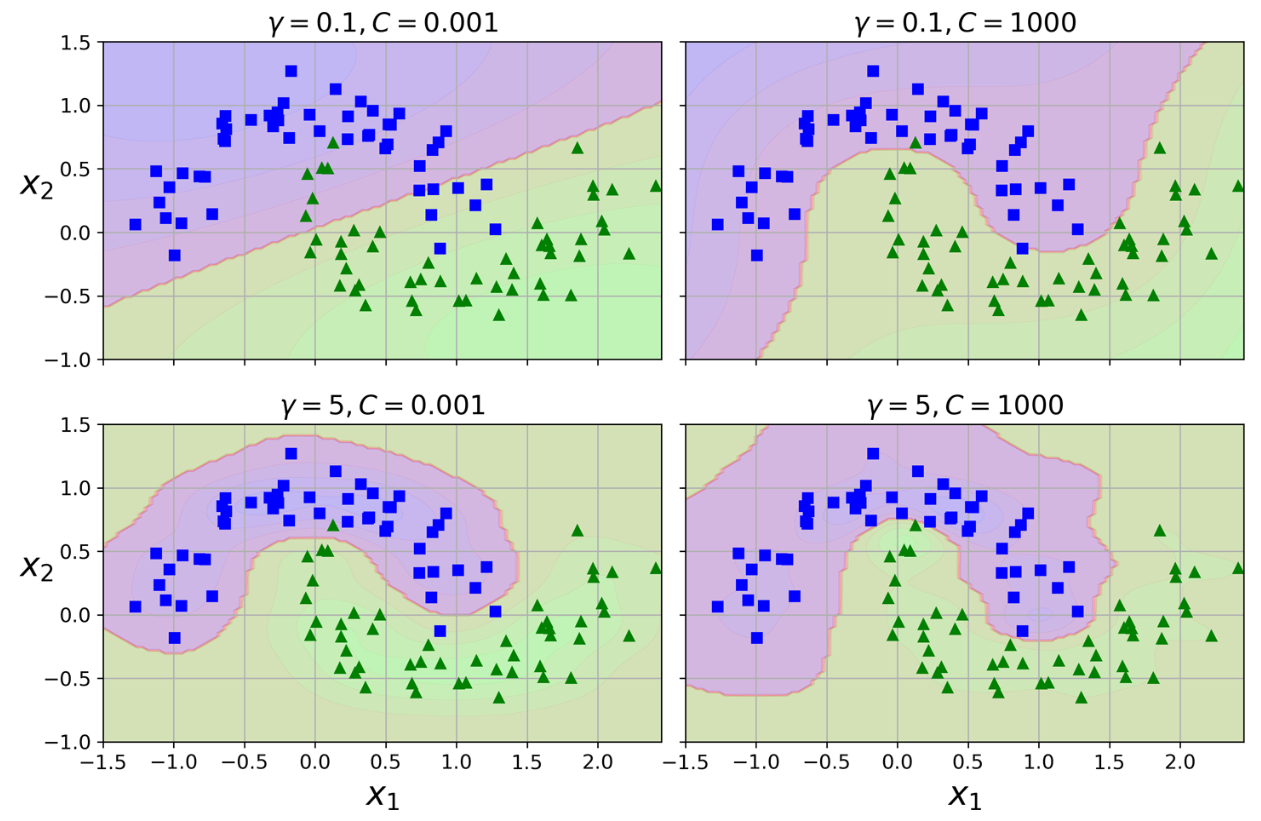
\includegraphics[scale=0.45]{Images/rbfKernel.PNG}

\noindent
There are other kernels that exist as well, but are used much more rarely. Some kernels are for specific data structures. For example, 
\textit{String Kernels} are sometimes used when classifiying documents or DNA sequences (e.g., using the \textit{string subsequence kernel}
or kernels based on the \textit{Levenshtein distance}).\\

\noindent
\textbf{As a Tip:}, one should always try the linear kernel first (remember that \mintinline{python}{LinearSVC} is much faster than 
\mintinline{python}{SVC(kernel="linear")}), especially is the training set is very large or if it has many features. Additionally, we can 
also try the Gaussian RBF kernel is the training set is not too large. Finally, it is never a bad idea to try and use a kernel specialized
whatever data structure that the training set may have.